\documentclass[11pt]{article}

\usepackage[ngerman]{babel}
\usepackage{amsmath}
\usepackage{calc}
\usepackage{csquotes}
\usepackage{graphics}
\usepackage{graphicx}
\usepackage{xcolor}
\MakeOuterQuote{"}
\usepackage[left=1cm,top=1.5cm,right=1.5cm, bottom=1cm]{geometry}
\usepackage{hyperref}
\usepackage{fancyvrb}


\setlength{\parindent}{0}

\begin{document}

    \section{CSS - Cascading Style Sheets}

    HTML ohne CSS ist langweilig.
    Wollen wir nicht nur einen schwarz-weiß Blob von Text und seltsam positionierten Bildern sehen,
    müssen wir mit CSS arbeiten.
    Letzten Endes ist CSS eine Ansammlung von Regeln, die wir auf HTML-Elemente anwenden können,
    um diese nach unseren Wünschen darstellen zu lassen.

    \subsection{Erste Schritte mit CSS}

    Um CSS zu nutzen, müssen wir zunächst in \Verb"<head>" Bereich unserer \Verb"index.html" einen CSS-Block anlegen:

    \begin{verbatim}
        <!DOCTYPE html>
        <html>
            <head>
                <style>
                     [hier kommt nachher unser CSS hin]
                </style>
            </head>
            <body>
                ...
            </body>
        </html>
    \end{verbatim}

    Innerhalb des \Verb"<style>" tags können wir unsere Regeln definieren um das Aussehen der Webseite zu beeinflussen.
    Das funktioniert ganz abstrakt immer so:

    \begin{verbatim}
        selektor {
            regel1: wert1;
            regel2: wert2;
        }
    \end{verbatim}

    Der Selektor gibt an, auf welches Element (oder welche Elemente) wir die Regeln innerhalb von \Verb"{\ldots}"
    anwenden wollen.
    Die erste Regel die wir ausprobieren wollen ist \Verb"color".
    Mit \Verb"color" legt man die \textit{Textfarbe} fest.

    Einfaches Beispiel:

    \begin{verbatim}
        ...
        <style>
           body {
               color: blue;
           }
        </style>
        ...
    \end{verbatim}

    Was steht da?
    Der Selektor ist \Verb"body", damit wird der Tag \Verb"<body>" selektiert.
    Man erinnere sich daran, dass ein HTML-Dokument immer als Baumstruktur aufgebaut ist.
    Wird eine Regel auf ein Element angewendet, so gilt diese (meistens) auch für alle Kindelemente (englisch Child-Elements)
    oder Unterelemente (alle Elemente, die in der Hierarchie "unter" diesem Element stehen).
    Das heißt, in unserem Beispiel bekommt sowohl \Verb"<body>" selbst, als auch jedes weitere Tag im \Verb"<body>" die
    Eigenschaft \Verb"color: blue".
    Probieren wir es aus: \newpage

    \begin{verbatim}
        ...
        <body>
            <p>Ich bin ein Abschnitt...</p>
            <p>Ich auch. Oh, wir sind ja blau!</p>
        </body>
        ...
    \end{verbatim}

    Beide Paragraphen (Absätze, also \Verb"<p>"-Tags) sollten blauen Text haben, da sie Kindknoten von \Verb"<body>" sind.
    Fügen wir eine weitere Regel in unserem CSS Code hinzu:

    \begin{verbatim}
        ...
        <style>
           body {
               color: blue;
           }

           p {
               color: red;
           }
        </style>
        ...
    \end{verbatim}

    Und erweitern unseren body wie folgt:

    \begin{verbatim}
        ...
        <body>
            <div>Banane</div>
            <p>Ich bin ein Abschnitt...</p>
            <p>Ich auch. Oh, wir sind nicht mehr blau!</p>
            <div>Maracuja</div>
        </body>
        ...
    \end{verbatim}

    Bevor wir speichern und die Seite neu laden: Was erwarten wir, was jetzt passiert? \\
    Nachdem wir uns das Resultat angeschaut haben: Ist uns klar, warum das so aussieht?

    \subsection{Klassen}

    Manchmal haben wir das gleiche HTML-Element mehrmals, wollen aber die einzelnen Elemente unterschiedlich
    stylen.
    Hier kommen Klassen ins Spiel.
    Jedes HTML-Tag kann zusätzlich \textit{Attribute} haben.
    Das ganze sieht so aus:

    \begin{verbatim}
        <tag attribut="wert">...</tag>
    \end{verbatim}

    Es gibt verschiedene Attribute, vielleicht ist das Attribut \Verb"src" des \Verb"<img>"-Tags bereits bekannt.
    Wir benötigen jetzt das Attribut namens \Verb"class".
    Diesem können wir einen beliebigen Wert geben, den wir anschließend im Stylesheet referenzieren können.
    Das geht wie folgt:

    \begin{verbatim}
        <body>
            <p class="abschnitt1">irgendein cooler text</p>
            <p class="abschnitt2">sonst was</p>
            <p class="abschnitt3">ok reicht langsam</p>
        </body>
    \end{verbatim}

    Wollen wir statt "jeden Tag mit diesem Namen" alle "Tags mit dieser Klasse" im CSS Code selektieren,
    machen wir das mit \Verb".klassen-name" (man beachte den Punkt am Anfang).
    Ersetzen wir unser bisheriges Stylesheet durch den folgenden Inhalt:

    \begin{verbatim}
        ...
        <style>
        .abschnitt1 {
            color: red;
        }

        .abschnitt2 {
            color: green;
        }

        .abschnitt3 {
            color: blue;
        }
        </style>
        ...
    \end{verbatim}

    Nun sollte jeder der drei Abschnitte eine eigene Farbe haben.

    \subsection{Farben in CSS}

    Farben können entweder mit einem englischen Begriff bezeichnet werden, eine Übersicht über alle
    verfügbaren Namen gibt es hier: \url{https://www.w3schools.com/cssref/css_colors.php}

    Man kann aber auch so jede beliebige (vom Monitor darstellbare) Farbe angeben:

    \begin{verbatim}
        body {
            background-color: rgb(100, 0, 100);
        }
    \end{verbatim}

    Welche Farbe erzeugt diese Regel?
    Warum?
    Wie lassen sich andere Farben damit darstellen?

    \newpage

    \subsection{Aufgaben}

    \begin{minipage}{0.4\textwidth}
            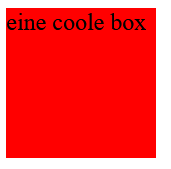
\includegraphics[width=2.5cm]{css1} \\
    \end{minipage}
    \hspace{0.1\textwidth}
    \begin{minipage}{0.4\textwidth}
        Hinweis: \Verb"<div>"-Element mit fester Größe \\

        neue CSS-Regeln:
        \begin{itemize}
            \item \Verb"width"
            \item \Verb"height"
            \item \Verb"background-color"
        \end{itemize}
    \end{minipage}

    \vspace{0.5cm}
    \hrule
    \vspace{0.5cm}

    \begin{minipage}{0.4\textwidth}
        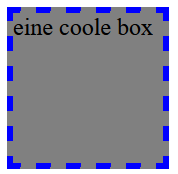
\includegraphics[width=2.5cm]{css2} \\
    \end{minipage}
    \hspace{0.1\textwidth}
    \begin{minipage}{0.4\textwidth}
        Hinweis: \Verb"<div>"-Element mit fester Größe \\

        neue CSS-Regeln:
        \begin{itemize}
            \item \Verb"border-color"
            \item \Verb"border-style"
            \item \Verb"border-width"
        \end{itemize}

        Wie kann man diese 3 Regeln unter einer Regel \Verb"border" zusammenfassen?
    \end{minipage}

    \vspace{0.5cm}
    \hrule
    \vspace{0.5cm}

    \begin{minipage}{0.4\textwidth}
        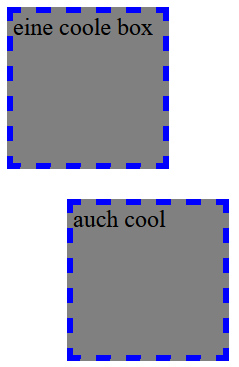
\includegraphics[width=2.5cm]{css3} \\
    \end{minipage}
    \hspace{0.1\textwidth}
    \begin{minipage}{0.4\textwidth}
        Hinweis: zwei mal das \Verb"<div>" aus der vorherigen Aufgabe \\

        neue CSS-Regeln:
        \begin{itemize}
            \item \Verb"margin-top"
            \item \Verb"margin-left"
            \item \Verb"margin-right"
            \item \Verb"margin-bottom"
        \end{itemize}


    \end{minipage}

    \vspace{0.5cm}
    \hrule
    \vspace{0.5cm}

    \begin{minipage}{0.4\textwidth}
        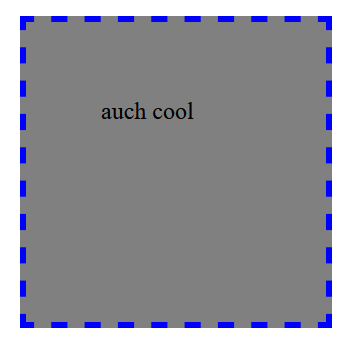
\includegraphics[width=2.5cm]{css4} \\
    \end{minipage}
    \hspace{0.1\textwidth}
    \begin{minipage}{0.4\textwidth}
        Hinweis: zwei mal das \Verb"<div>" aus der vorherigen Aufgabe \\

        neue CSS-Regel:
        \begin{itemize}
            \item \Verb"padding"
        \end{itemize}


    \end{minipage}

    \vspace{0.5cm}
    \hrule
    \vspace{0.5cm}

    \begin{minipage}{0.4\textwidth}
        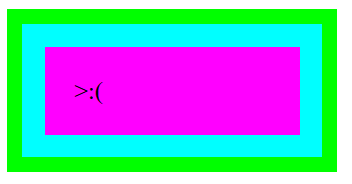
\includegraphics[width=3.5cm]{css5} \\
    \end{minipage}
    \hspace{0.1\textwidth}
    \begin{minipage}{0.4\textwidth}
    \end{minipage}

    \vspace{0.5cm}
    \hrule
    \vspace{0.5cm}

    \begin{minipage}{0.4\textwidth}
        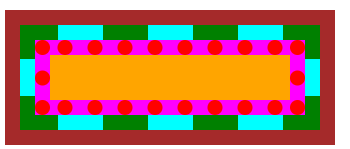
\includegraphics[width=3.5cm]{css6} \\
    \end{minipage}
    \hspace{0.1\textwidth}
    \begin{minipage}{0.4\textwidth}
        Hinweis: border\dots \\
    \end{minipage}

    \vspace{0.5cm}
    \hrule
    \vspace{0.5cm}

    \begin{minipage}{0.4\textwidth}
        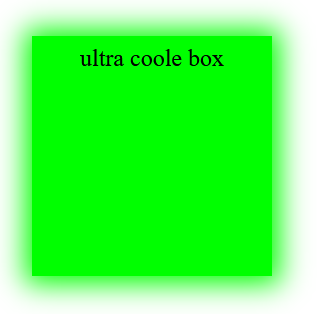
\includegraphics[width=4.5cm]{css7} \\
    \end{minipage}
    \hspace{0.1\textwidth}
    \begin{minipage}{0.4\textwidth}
        neue CSS-Regel:
        \begin{itemize}
            \item \Verb"box-shadow"
        \end{itemize}
    \end{minipage}

    \vspace{0.5cm}
    \hrule
    \vspace{0.5cm}

    \begin{minipage}{0.4\textwidth}
        
\includegraphics[width=4.5cm]{css9} \\
    \end{minipage}
    \hspace{0.1\textwidth}
    \begin{minipage}{0.4\textwidth}
        Neue CSS-Regeln:
        \begin{itemize}
            \item \Verb"font-weight"
            \item \Verb"font-family"
            \item \Verb"font-size"
            \item \Verb"text-shadow"
        \end{itemize}
    \end{minipage}

    \vspace{0.5cm}
    \hrule
    \vspace{0.5cm}

    \begin{minipage}{0.4\textwidth}
        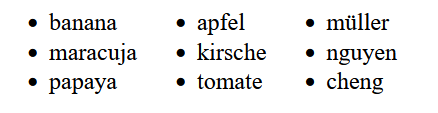
\includegraphics[width=4.5cm]{css8} \\
    \end{minipage}
    \hspace{0.1\textwidth}
    \begin{minipage}{0.4\textwidth}
        Hinweis: flex-layout. \\
        Am besten kurz melden, wenn ihr hier angekommen seid.
    \end{minipage}

    \vspace{0.5cm}
    \hrule
    \vspace{0.5cm}

\end{document}
